\section{Metod} 

Nedan följer en beskrivning av de arbetsmetoder, mjukvaror och kodbibliotek som vi använt oss av i projektet. 

\subsection{Genomförande}

% modulbaserat arbete..
För att implementera en tolk för Haskell behövs en parser för den aktuella syntaxen, en typcheckare för språkets definierade typregler och tillsist en interpretator som tolkar språket efter dess specifikation.
Det upptäcktes tidigt att de tre modulerna, parser, interpretator och typcheckare inte behövde utvecklas sekvensiellt. De tre modulerna integrerar enbart med varandra genom det abstrakta syntaxträdet, vår interna representation av Haskell, vilket medför att det är lätt att utveckla de olika modulerna helt frånskilt från varandra. Figur \ref{fig:tolkens_struktur} visar hur denna interaktion mellan de olika modulerna är tänkt att gå till. Figuren visar även hur webbläsaren kommunicerar genom ett Javascript API och det abstrakta syntaxträdet och inte direkt med de olika komponenterna. 

\begin{figure}[h]
    \begin{center}
        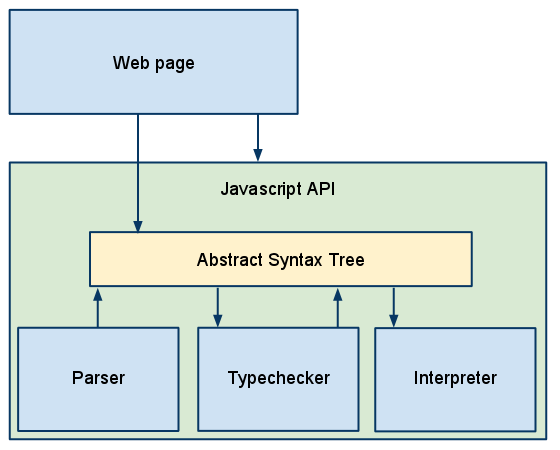
\includegraphics[width=1.0\textwidth]{image1.png}
        \caption{Överblick över tolkens struktur och interaktion}
        \label{fig:tolkens_struktur} % Labels must come after caption!
    \end{center}
\end{figure}

Det första delmålet var att göra en haskelliknande implementation av lambda calculus då mer avancerade funktionella programspråksegenskaper kan implementeras som detta \citep{jones87}.
Parsern implementerades med hjälp av ett \emph{parser combinator}-bibliotek kallat JSParse \citep{jsparse}. Det gav oss möjlighet att på ett enkelt sätt implementera både den kontextfria och icke kontextfria delen av Haskell. Parsern skapar ett syntaxträd som skickas vidare till typcheckaren. I typcheckaren dekoreras syntaxträdet med typinformation innan det slutligen skickas till interpretatorn.

En interaktiv kommandotolk som kan köras i en webbläsare utvecklades. Den gav användaren möjlighet att skriva haskellfunktioner och exekvera dem på ett liknande sätt som i GHCi. 
Vi integrerade jQuery \citep{jquery} för att få ett unisont stöd för samtliga webbläsare. jQuery underlättade även arbetet med att skapa ett enkelt och stilrent interaktivt gränssnitt.

Arbetssättet präglades av en iterativ utvecklingsmetodik med korta utvecklingscyklar. Arbetet delades upp med huvudansvarstagande över var sin modul och utfördes parallellt med varandra. Arbetet skedde dock framförallt i samlad grupp på grund av att det var många designrelaterade problem vi var tvungna att ta ställning till under projektet, till exempel hur vårt abstrakta syntaxträd skulle se ut, och för att det skulle bli enklare när vi skulle börja sammanfoga de olika modulerna med varandra. 
Det var också ett bra sätt att snabbt få hjälp av varandra eftersom vi ej visste exakt hur modulerna skulle se ut när vi påbörjade arbetet. Vi fann det därför praktiskt att använde en iterativ modell för att bit för bit utvidga våra moduler. Dock valde vi att implementera typcheckaren i ett steg då vi ansåg att det skulle vara enklare. Detta främst för att vi trodde typklasser var så centralt i typcheckaren att det skulle vara svårt att lägga till det i en andra iteration. 

Eftersom vi arbetade parallellt med olika moduler var vi beroende av ett bra versionshanteringssystem. Bra i vårt fall innebar att det skulle vara enkelt att arbeta i olika grenar, en gren för varje modul, och att det skulle gå snabbt och enkelt att slå ihop dessa förgreningar när vi behövde länka samman två utvecklares arbeten. I början av projektet använda vi oss av Subversion (SVN). Detta berodde framförallt på att det var det versionshanteringssystem som alla i gruppen hade erfarenhet från tidigare. Dock insåg vi att SVN inte var praktiskt att använda när vi arbetade i flera olika grenar i projektet samtidigt. Därför gick valet till att använda Git som är designat från grunden för att på ett enkelt sätt skapa nya och slå samman förgreningar under utvecklingens gång. Vi kunde därmed skapa en förgrening för varje modul och under arbetets gång sammanlänka allas arbeten på ett effektivt sätt. 

På grund av vår parallella arbetsmetod ansåg vi det nödvändigt att arbeta fram en kodstandard så att de olika modulerna skulle stilmässigt likna varandra. Kodstandarden beskriver hur indentering och namngivning av variabler och funktioner ska se ut. Innan ny kod skickades till Git så krävdes det att koden uppfyllde kraven i kodstandarden.  

%\subsection{Javascript} 
%Javascript \citep{javascript} är ett programmeringsspråk som framförallt används på klientsidan på webben. Javascript är ett dynamiskt objektorienterat skriptspråk.
%Javascript är det programmeringsspråk som används uteslutande i detta projektet.

\subsection{Kodbibliotek}
I projektet använder vi oss av tre kodbibliotek för att snabbare kunna utveckla haskelltolken. Nedan följer en kort beskrivning av dessa.

\subsubsection{JSParse}  
Parsern implementeras med hjälp av ett parser combinator bibliotek kallat JSParse. 
En parser combinator består av olika funktioner som parsar exempelvis strängar, listor eller blanksteg.
Dessa funktioner kombineras för att skapa mer komplexa parsers. Det ger oss möjlighet att implementera komplexa
parsers för både de kontextfria och icke kontextfria varianterna av Haskell.

\subsubsection{jQuery} 
%jQuery är ett öppet kodbibliotek till Javascript som är dubeellicenserat under MIT License och GPL version 2.  
jQuery är designat för att underlätta för utvecklare att modifiera DOM-träd och göra asynkrona javascriptanrop jQuery användes i projektet för att få likartat stöd i samtliga webbläsare i kommandotolken som utvecklades. 
jQuery gav oss även möjlighet att skapa ett enkelt och stilrent interaktivt gränssnitt utan att behöva göra allt från grunden.
jQuery.Cookie, ett tillägg till jQuery, används för att förenkla användandet av kakor.

\subsubsection{JSON}
JSON \citep{json}  är en delmängd av Javascript och används för att utbyta data mellan olika format och programmeringsspråk. 
JSON är idag inbyggt i de senaste versionerna av de moderna webbläsarna, men för att få stöd i äldre versioner har vi valt att inkludera JSON som ett externt bibliotek.

